\section{Introduction}

A large body of evidence from human and other primate studies 
suggest that they use reinforcement signals to learn tasks and reinforcement 
learning has proved to be a good model for this process.
However humans are able to learn and carry out very complex tasks involving 
many different objectives. 
How can they do this? The likelihood is that they use reinforcement in this 
context as well but most formal reinforcement learning models do not scale 
well with increasing complexity.

One promising possibility is that the complex task can be broken down into 
sub-tasks that are each learned separately \cite{sprague2003multiple,
rothkopf2013modular, dietterich2000hierarchical}. 
For certain task venues, this decomposition allows the behavior in the complex 
task to be specified as a weighted sum of individual sub-task priorities.
This paper explores the use of such a decomposition to characterize complex
behavior of subjects in a virtual reality environment. The methodology of
\cite{rothkopf2013modular} allows the task priorities to be estimated using the
subjects' behavioral data.

Our experimental analysis shows that the modular reinforcement can be a 
surprisingly good model of behavior, predicting individual subjects' sub-task 
priorities in a way that explains their behavioral choices.

This paper is organized as follows. Section~\ref{sec:domain} introduces the
domain of the composite task that we collected human data. Section~\ref{sec:rl}
describes the main algorithm, modular inverse reinforcement learning. We report
our experiment results in Section~\ref{sec:exp}, and conclude in
Section~\ref{sec:conclude}.

\section{Multi-objective Domain}
\label{sec:domain}

\begin{figure}[h!]
\centering
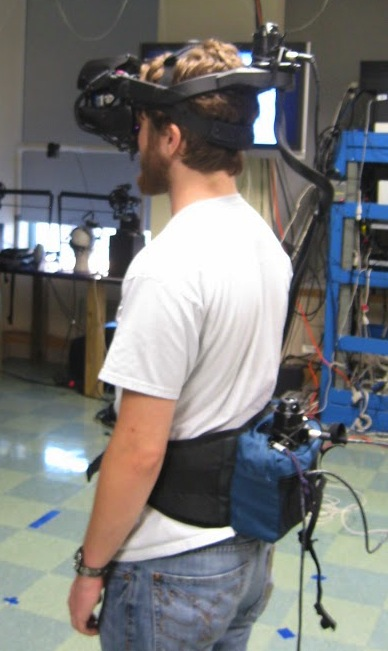
\includegraphics[height=5cm]{human.jpg}
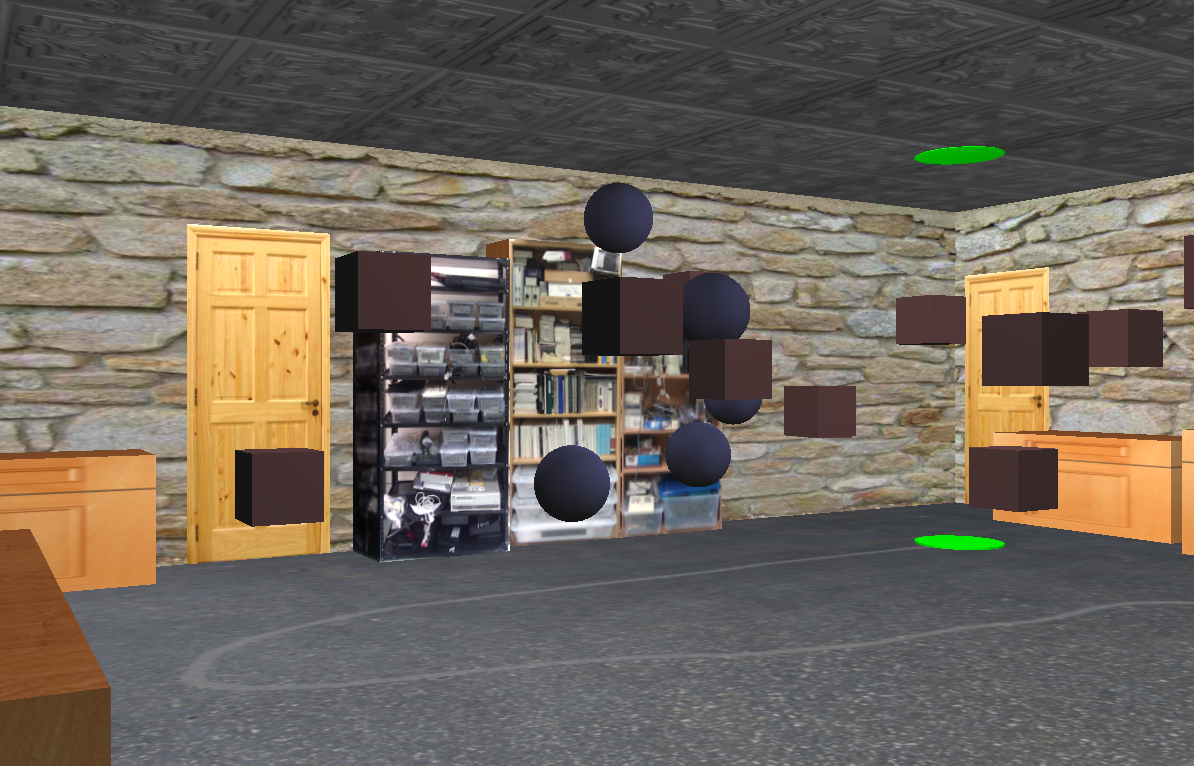
\includegraphics[height=5cm]{env.png}
\caption{(Left) A human subject with head tracker, virtual reality displayer, and
body tracker.  (Right) The environment the human can see through the displayer.
The red cubes represent obstacles. The blue balls represent targets. There is
also a gray path on the ground that the human subject can follow.}
\label{fig:avatar}
\end{figure}

Figure~\ref{fig:avatar} shows the domain that we used for our experiment. The
agent, which is a human subject in this case, is in a virtual reality domain.
We ask the human subject to have trackers and a virtual reality displayer
equipped. He can see the environment through the displayer in front of his eyes,
and he can walk as if he is walking in the virtual domain.
The agent would be punished if running into obstacles (red cubes), and rewarded
if collecting targets (blue balls). There is a path on the ground that he can
follow.
Naturally, this domain has three sub-tasks, 1) following the path, 2)
collecting targets, 3) avoiding obstacles.
This is an experiment used in the literature to evaluate modular reinforcement
learning \cite{rothkopf2013modular} and understand human behavior \cite{Tong2014}.

We will evaluate four different tasks. {\bf Task 1}, following the path only, and
ignoring other objects. {\bf Task 2}, following the path, while avoiding the obstacles.
{\bf Task 3}, following the path, while collecting targets when possible. {\bf Task 4},
following the path, collecting the targets and avoiding obstacles
simultaneously.
We conducted experiments to ask human subjects to accomplish these tasks and
recorded their trajectories. The human data are collected by the Center for
Perceptual Systems at University of Texas at Austin.

If the agent observes the distance and angle to an object, he is expected to
know the optimal action to avoid or pursue it. This decision is also Markov.
Therefore, the question would be, if we have trained modules for these three
sub-tasks, could they be integrated to match human's behavior?

\section{Modular Inverse Reinforcement Learning}
\label{sec:rl}

Recall that for a state, action
pair, $s$ and $a$, $Q(s, a)$ evaluates the utility of taking action $a$ from
state $s$. The {\em policy} of a state is the action with the maximum Q
value \cite{rl}. So how do we determine the global policy from the modules, or
sub-tasks? In the literature, work has been done to integrate the decomposed
value functions of the sub-tasks \cite{koller1999computing}. The sub-tasks can
also propose their own policies, while the global policy is a weighted sum of
those sub-task policies \cite{thomas2012motor}.

Here, we assume that the global Q function is a weighted sum of all $Q_i$, where
$Q_i$ is the Q function for i-th module.
$$Q(s, a) = \sum_i w_i Q_i (s_i, a)$$
where $w_i$ is the weight of the i-th sub-MDP. $w_i \geq 0, \sum_i w_i = 1$.
$s_i$ denotes the decomposition of $s$ in the i-th module.

Different weights can yield different performance. Let $w$ be the vector of
$(w_1, w_2, w_3)$, where $w_1, w_2, w_3$ are weights for the sub-tasks of target
collection, obstacle avoidance, and path following, respectively. An agent with
$w = (1, 0, 0)$ only collects targets, and one with $w = (0, 0.5, 0.5)$ may
avoid the obstacles and follow the path.

To obtain the weights given the samples, we need to use the inverse
reinforcement learning technique. In reinforcement learning, we derive 
optimal policies given an MDP. In inverse reinforcement learning, however, we
find out the underlying MDP by observing policies. In the literature, a common
way is to use a maximum likelihood method to recover the transition function and
the reward function \cite{ng2000algorithms}. Here, however, we only need to find
out the weights. The transition function is known, and the reward function is
trivially the weighted sum of that of modules. Concretely, we use the modular
inverse reinforcement learning method \cite{rothkopf2013modular} to maximize the
function below.
\begin{equation}
\label{eq:irl}
\max_w \prod_t \frac{e^{\eta Q(s^{(t)}, a^{(t)})}}{\sum_b e^{\eta Q(s^{(t)}, b)}}
\end{equation}
where $s^{(t)}$ is the state at time $t$, and $a^{(t)}$ is the action at time
$t$, which are both from samples. $Q(s, a) = \sum_i w_i Q_i(s_i, a)$, as defined
before. $\eta$ is a hyperparameter that determines the consistency of human's
behavior. The larger $\eta$ is, the algorithm is more likely to overfit the data.

The intuition of Equation~\ref{eq:irl} is that if an action is observed from the
sample, then the Q value of taking that action should be larger compared to Q
values of taking other actions.

\section{Experiments}
\label{sec:exp}

We trained the modules first to obtain $Q_i$ before running the inverse reinforcement
learning algorithm. For each module, the agent only considers the closest target
and the closest obstacle. For the path module, the path is defined as segments
connected by waypoints, so the next waypoint is considered. The agent takes the
distance and angle to the closest objects as the state representation.

To make our weights represent the significance of the modules, we
normalize the sub-MDPs with the unit (positive or negative) reward. The reward
is 1 for collecting a target, -1 for running into an obstacle, and 1 for
collecting a waypoint of the path. In the implementation, we make the radius of
waypoints larger than that of other objects, so that the agent will not cling
too much to the path.

We make some constraints on our learning agent to make it walk like a human.
We can find from the human trajectories that humans walk smoothly and do not turn
sharply.  Our agent is only allowed to do three actions --- going straight ahead,
turning left with a small step, and turning right with a small step.

\begin{figure}[h]
\centering
\begin{subfigure}[b]{0.24\textwidth}
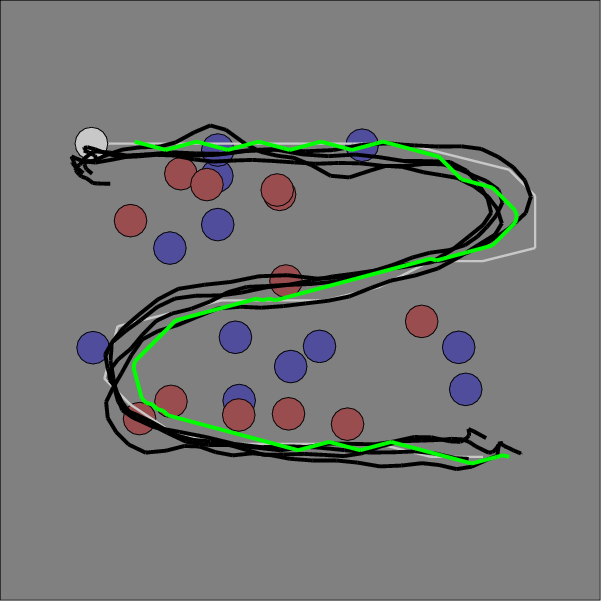
\includegraphics[width=\textwidth]{task_1.png}
\caption{Path module only,\\$w = (0.039, 0.0, 0.960)$. }
\end{subfigure}
\begin{subfigure}[b]{0.24\textwidth}
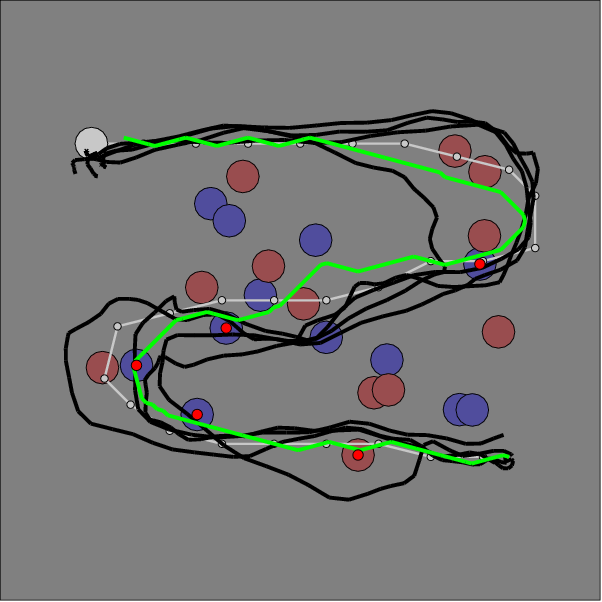
\includegraphics[width=\textwidth]{task_2.png}
\caption{Obstacle + Path,\\$w = (0.081, 0.264, 0.654)$. }
\end{subfigure}
\begin{subfigure}[b]{0.24\textwidth}
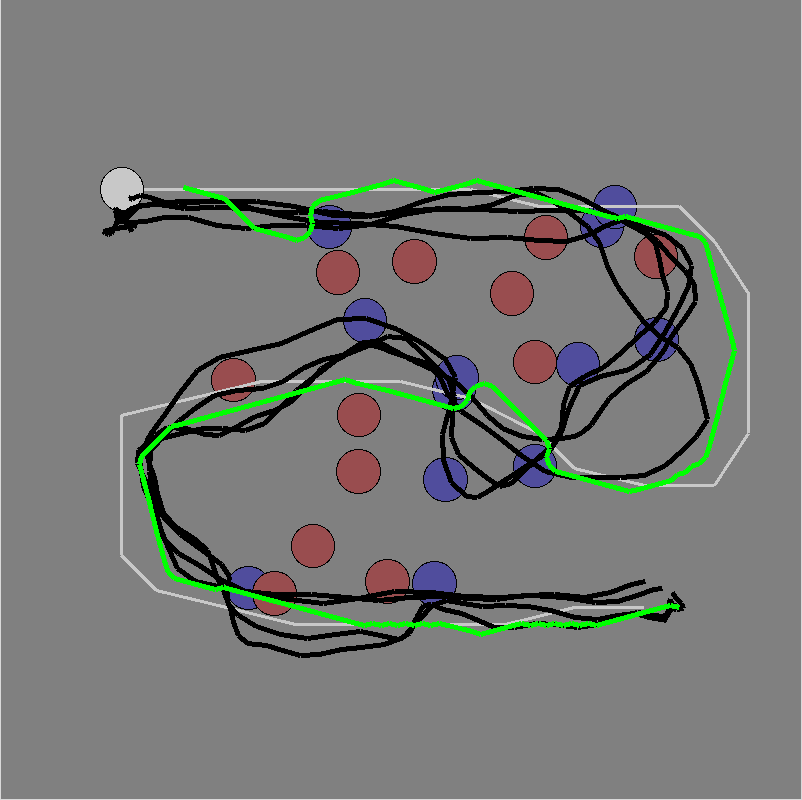
\includegraphics[width=\textwidth]{task_3.png}
\caption{Target + Path, \\$w = (0.254, 0.089, 0.655)$. }
\end{subfigure}
\begin{subfigure}[b]{0.24\textwidth}
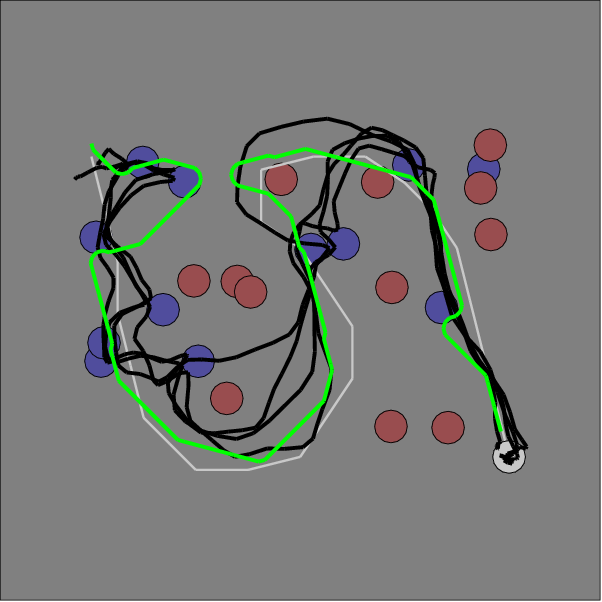
\includegraphics[width=\textwidth]{task_4.png}
\caption{Target + Obstacle + Path, \\$w = (0.215, 0.414, 0.369)$. }
\end{subfigure}
\caption{The trajectories of humans and the agent in the four tasks. The
black lines are trajectories of human subjects, and the green lines are
trajectories of the learning agent by using the optimum weights, $w$, derived
from modular inverse reinforcement learning. Weights are shown in the target,
obstacle, path order.}

\label{fig:exp}
\end{figure}

\begin{figure}[h]
\centering
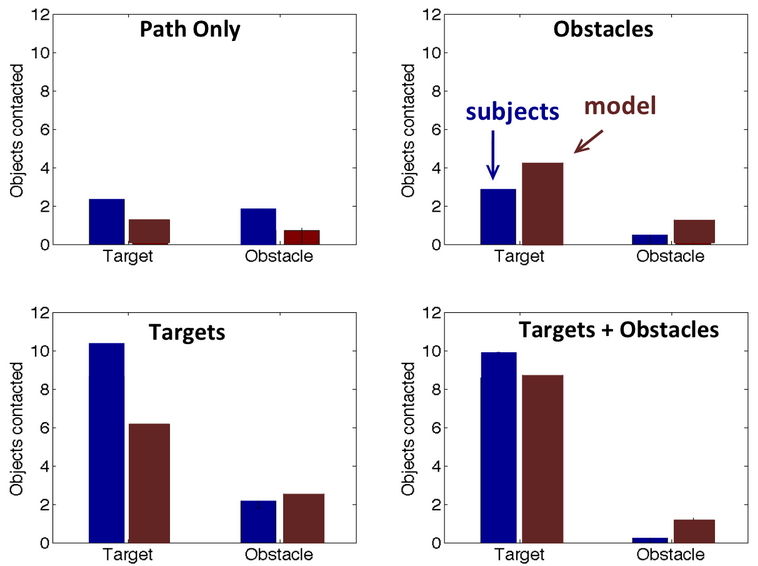
\includegraphics[width=0.5\textwidth]{contactStats.png}
\caption{Number of targets hit and number of obstacles hit of the human subjects
and the agent.}
\label{fig:stats}
\end{figure}

We report the results in Figure~\ref{fig:exp}. Same as Figure~\ref{fig:avatar},
the red circles are obstacles. The blue circles are targets. The gray lines are
the path. The black lines are trajectories of human --- each line represents one
human trajectory.
Using the weights derived from the algorithm, the trajectories of the agents are
drawn in green color.

Although humans don't agree with each other on how to avoid obstacles or collect
targets, the agent can figure out what the humans are doing, and perform a
similar behavior. Figure~\ref{fig:stats} evaluates the
performance by showing the number of targets hit and number of obstacles hit.
The number of targets hit should be large, and the number of obstacles hit
should be small, when the corresponding module is active.
We can observe that humans still do better than the agent in these tasks.
Nevertheless, the agent has a similar performance compared to human subjects.

\begin{figure}[h]
\centering
\begin{subfigure}[b]{0.4\textwidth}
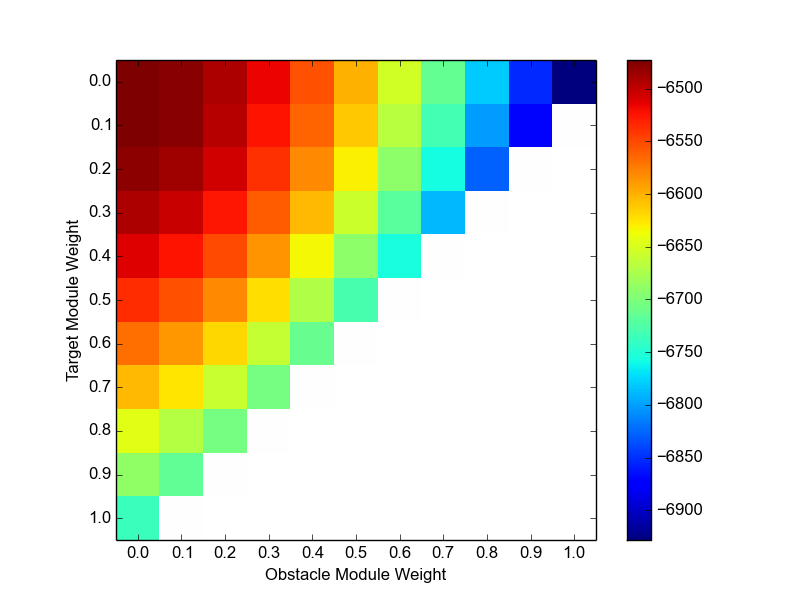
\includegraphics[width=\textwidth]{objValuesTask1.png}
\caption{Path following only.}
\end{subfigure}
\begin{subfigure}[b]{0.4\textwidth}
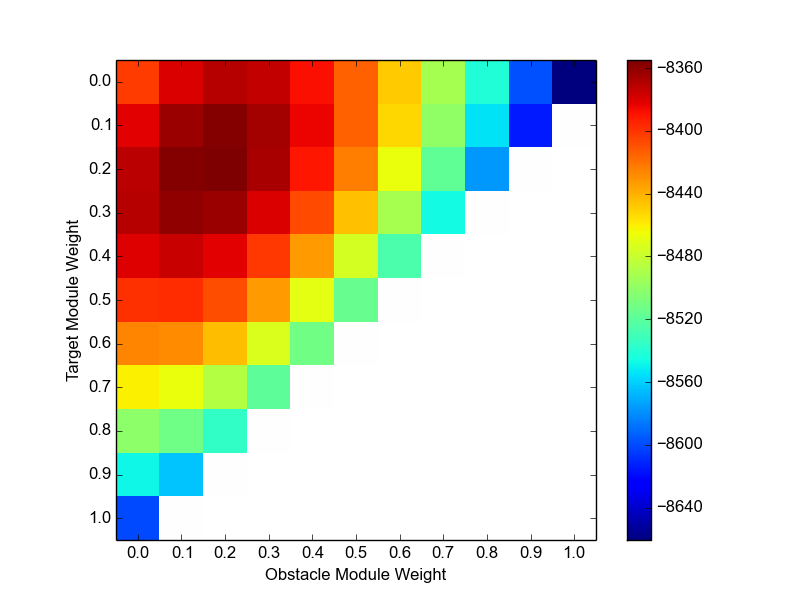
\includegraphics[width=\textwidth]{objValuesTask2.png}
\caption{Obstacle + Path. }
\end{subfigure}
\begin{subfigure}[b]{0.4\textwidth}
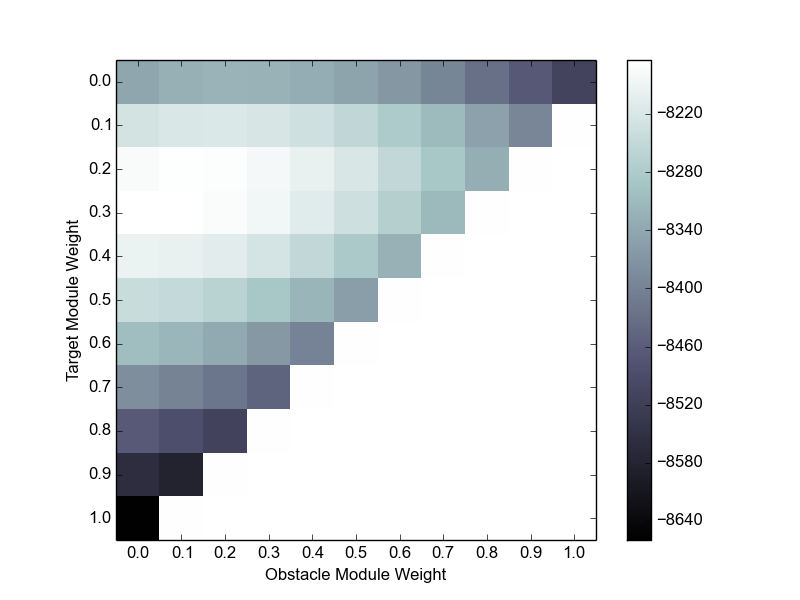
\includegraphics[width=\textwidth]{objValuesTask3.png}
\caption{Target + Path. }
\end{subfigure}
\begin{subfigure}[b]{0.4\textwidth}
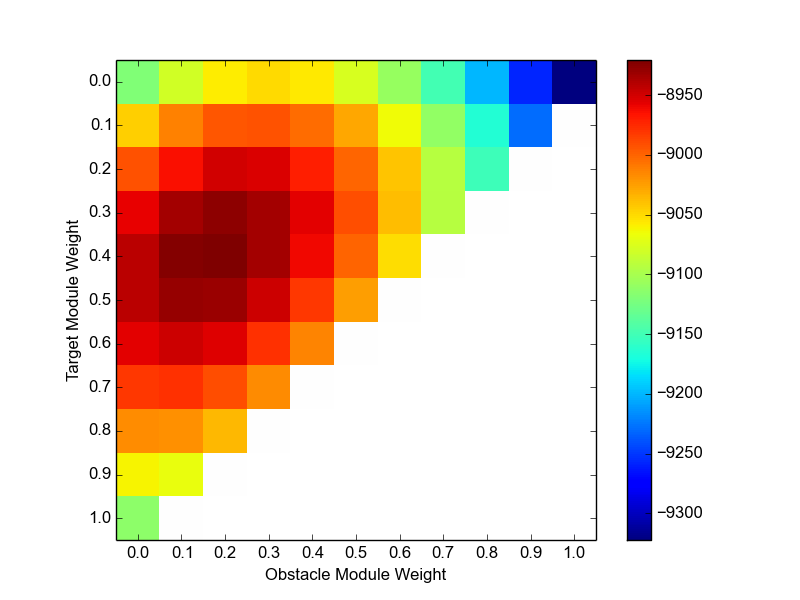
\includegraphics[width=\textwidth]{objValuesTask4.png}
\caption{Target + Obstacle + Path. }
\end{subfigure}
\caption{Heatmaps of the $\log$ of the values of Equation~\ref{eq:irl} for
different weights for the four tasks, respectively. The white zones indicate
higher probabilities. The weights of all three modules sum to 1, so we only show
the weights on the target and the obstacle modules.
}
\label{fig:heatmap}
\end{figure}

In Figure~\ref{fig:heatmap}, we show the $\log$ of values of
Equation~\ref{eq:irl} for different weights. The white color represents higher
probability. We can observe the centroids of white zones move for different
tasks. It stays at the origin in Task 1, so none of the target module and
obstacle module is active. It moves away from the origin when a module is
active.  From the heatmaps, we find the optimums exist for these tasks. The
optimal weights are also consistent with the experiment context.

\section{Conclusion and Future Work}
\label{sec:conclude}

We interpreted human behavior using inverse module reinforcement learning in
this paper. The experimental results show that modular reinforcement learning
can well explain human behavior, even though the performance of the agent is
inferior to human subjects'.

There are also some observations potential for the future work. First, 
weighted sum of Q functions is one way to combine multiple sub-MDPs. We also
propose other ways including, for example, scheduling between different modules,
with only one active at one time. This is also called {\em skill} in the literature
\cite{konidaris2009skill}. However, we adopt the weighted sum approach
because this is more reasonable for human behavior. When a human tries to collect
targets while avoiding obstacles, these two modules are expected to be both
active. A scheduling approach may yield frequent oscillation between these two
modules.

Second, we also assume independency between modules. Correlation between
modules doesn't impair our analysis in this paper. In Figure~\ref{fig:heatmap},
we can tell that the target module and obstacle module tend to be negatively
correlated from the shape of the white zones.

Lastly, weights may be dynamic and different from state to state. However, with
such assumption, we need to learn a mapping from state to weights. In this case,
the curse of dimensionality still exists, and inverse learning would be
difficult.


